% Agentic System Design Process -- hand-maintained source (see README.md).
\documentclass[10pt]{article}
\usepackage[T1]{fontenc}
\usepackage[utf8]{inputenc}
\usepackage{lmodern}
\usepackage[letterpaper,margin=2.2cm]{geometry}
\usepackage{microtype}
\usepackage{xcolor}
\usepackage{array,booktabs,tabularx}
\usepackage{enumitem}
\usepackage{amssymb}
\usepackage{parskip}
\usepackage[most]{tcolorbox}
\usepackage[colorlinks=true,linkcolor=blue!55!black,urlcolor=teal!55!black,citecolor=blue!55!black]{hyperref}

\usepackage{tikz}
\usetikzlibrary{arrows.meta,backgrounds,calc}

\setlist{itemsep=1pt,topsep=2pt}

% Diagram style:
% pale panel, white boxes with thin grey rules, small monospace tags,
% one coral accent for the focal element, legend strip at the bottom.
\definecolor{dpbg}{HTML}{F3F4F6}
\definecolor{dpline}{HTML}{C3C8CF}
\definecolor{dpink}{HTML}{2B2F36}
\definecolor{dpmute}{HTML}{6B7280}
\definecolor{dpcoral}{HTML}{E2683C}
\definecolor{dpcoralbg}{HTML}{FBE4DA}
\newcommand{\dpmono}{\fontfamily{zi4}\selectfont}
\newcommand{\dptag}[1]{{\dpmono\tiny\color{dpmute}\MakeUppercase{#1}}}
\tikzset{
  dp/.style={font=\sffamily\scriptsize, color=dpink, >={Stealth[length=4pt,width=3.5pt]},
    show background rectangle, inner frame xsep=10pt, inner frame ysep=8pt,
    background rectangle/.style={fill=dpbg, draw=none},
    every node/.append style={execute at begin node={\hyphenpenalty=10000\exhyphenpenalty=10000}}},
  box/.style={draw=dpline, fill=white, line width=0.5pt, rounded corners=1.5pt, align=center, inner sep=4pt},
  focal/.style={box, draw=dpcoral, fill=dpcoralbg},
  hub/.style={box, draw=dpink, fill=dpink, text=white},
  flow/.style={->, draw=dpink, line width=0.6pt},
  back/.style={->, draw=dpmute, dashed, line width=0.6pt},
  hot/.style={->, draw=dpcoral, line width=0.7pt},
  lab/.style={font=\dpmono\tiny, text=dpmute, inner sep=1.5pt},
}
% \phbox{index}{x}{title}{style}: one phase card for the process map
\newcommand{\phbox}[4]{%
  \node[#4, minimum width=1.5cm, minimum height=1.95cm] (p#1) at (#2,0) {};
  \node[anchor=north, align=center, text width=1.42cm, inner sep=0pt] at ([yshift=-5pt]p#1.north)
    {\dptag{phase 0#1}\\[3pt]\textbf{#3}};}
\newcolumntype{L}{>{\raggedright\arraybackslash}X}

% Phase heading and boxes
\newcommand{\phase}[2]{\section*{Phase #1: #2}\addcontentsline{toc}{section}{Phase #1: #2}}
\newtcolorbox{goal}{colback=blue!4,colframe=blue!45!black,boxrule=0.5pt,arc=1pt,left=4pt,right=4pt,top=2pt,bottom=2pt}
\newtcolorbox{gate}{colback=green!5,colframe=green!40!black,boxrule=0.5pt,arc=1pt,left=4pt,right=4pt,top=2pt,bottom=2pt,title=Done when,fonttitle=\sffamily\bfseries\small}
\newcommand{\inferred}{\textsf{\small[inferred]}}

\title{\textbf{Agentic System Design Process}\\[4pt]
\large Nine phases from problem to production, assembled from the course materials and practitioner guides}
\author{J. A. Arroyo}
\date{Version 1.9 --- 14 October 2026 (appendix of worked examples)}

\begin{document}
\maketitle

\begin{abstract}
\noindent I did not find a complete lifecycle process in the public materials reviewed from the fifteen courses indexed in the guide \cite{guide}.
Individual courses cover some phases explicitly, through project templates, rubrics and slides, and the practitioner guides from Anthropic, OpenAI and Google cover most of the rest.
This document combines those sourced practices with my synthesis.
\textbf{The phase order, the gates and the resolutions between sources are inferred recommendations; the citations identify support for individual practices.}
Places where the sources differ are stated, not hidden.
\inferred{} marks a statement that the cited sources do not explicitly prescribe.
\end{abstract}

\tableofcontents

\section*{How to use this document}
\addcontentsline{toc}{section}{How to use this document}

\begin{tcolorbox}[colback=black!3,colframe=black!35,boxrule=0.4pt,arc=1pt,left=4pt,right=4pt,top=2pt,bottom=2pt,title={One set of three documents},fonttitle=\sffamily\bfseries\small]
\small
\begin{enumerate}[leftmargin=1.4em,itemsep=0pt]
\item \textbf{Learning to Build Agentic Systems} (the guide): the courses, lectures and assignments behind the practices. \emph{Use it to learn a topic.}
\item \textbf{Agentic System Design Process}: nine phases from framing a problem to running it in production. \emph{Use it to design a system.}
\item \textbf{Screening Tasks for Agentic Automation}: a one-page worksheet, filled in after Phase~1 of the design process, that feeds Phase~2 and sets up the comparison run in Phase~7. \emph{Use it to decide whether a task is worth it.}
\end{enumerate}
This is document~2. The courses it cites are indexed in the guide; the worksheet it uses in Phase~2 is in the screening companion \cite{screen}.
\end{tcolorbox}

Work the phases in order, and write down the output of each phase before moving on.
The process is not linear in practice:
\begin{itemize}
\item Between Phase~1 and Phase~2, fill in the screening worksheet \cite[Section~6]{screen}. Its answers are the input to Phase~2, and its last row is the comparison that Phase~7 runs.
\item Phase~7 can send you back to Phase~2 (simplify) or Phase~3 (re-split the work).
\item Phase~9 triages production failures and adds representative regression cases to the Phase~4 set.
\item Safety is not a late add-on. It is designed in Phases 1, 3 and 5 and tested in Phase~8.
\end{itemize}
Scale each phase to the stakes. For a small internal tool, a phase can be a paragraph; for a customer-facing system, it is a reviewed document.
The appendix works three examples through the worksheet and the phases.

\begin{center}
\small
\begin{tabularx}{\linewidth}{@{}r p{4.3cm} L l@{}}
\toprule
\# & Phase & Output & Support \\
\midrule
1 & Frame the problem & Problem brief with success and unacceptable failures & Strong \\
2 & Decide whether an agent is warranted & Option comparison; written justification & Strong (guides) \\
3 & Decompose and assign ownership & Task map: code / model / human; stop and approval points & Strong \\
4 & Define the evaluation & Test set, metrics, baseline, release bar & Very strong \\
5 & Design tools, state and context & Tool contracts, state model, permission boundaries & Strong \\
6 & Prototype and select models & One traced working path; model comparison & Practices strong; order disputed \\
7 & Evaluate, diagnose, iterate & Error analysis; improvements vs.\ baseline & Very strong \\
8 & Harden safety and approve release & Adversarial results; release sign-off & Strong \\
9 & Deploy gradually and maintain & Versioned rollout, monitoring, regression growth & Strong (guides); weak (courses) \\
\bottomrule
\end{tabularx}
\end{center}

Figure~\ref{fig:map} shows the phases, the return paths and where safety work happens.

\begin{figure}[htbp]
\centering
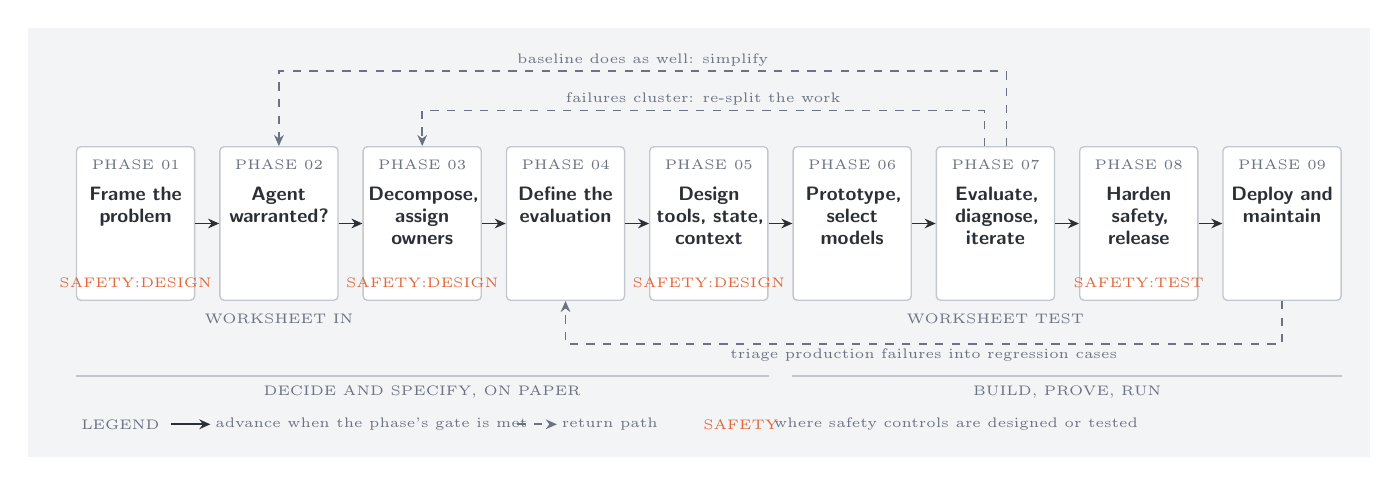
\begin{tikzpicture}[dp]
\def\dx{1.82}
\phbox{1}{0*\dx}{Frame the problem}{box}
\phbox{2}{1*\dx}{Agent warranted?}{box}
\phbox{3}{2*\dx}{Decompose, assign owners}{box}
\phbox{4}{3*\dx}{Define the evaluation}{box}
\phbox{5}{4*\dx}{Design tools, state, context}{box}
\phbox{6}{5*\dx}{Prototype, select models}{box}
\phbox{7}{6*\dx}{Evaluate, diagnose, iterate}{box}
\phbox{8}{7*\dx}{Harden safety, release}{box}
\phbox{9}{8*\dx}{Deploy and maintain}{box}
\foreach \i in {1,3,5} \node[lab, text=dpcoral, above=3pt] at (p\i.south) {SAFETY:DESIGN};
\node[lab, text=dpcoral, above=3pt] at (p8.south) {SAFETY:TEST};
\foreach \i/\j in {1/2,2/3,3/4,4/5,5/6,6/7,7/8,8/9} \draw[flow] (p\i.east) -- (p\j.west);
\node[lab, anchor=north] at ([yshift=-3pt]p2.south) {WORKSHEET IN};
\node[lab, anchor=north] at ([yshift=-3pt]p7.south) {WORKSHEET TEST};
% return paths above the row
\draw[back] ([xshift=-4pt]p7.north) -- ++(0,0.45) -| node[lab, pos=0.25, above] {failures cluster: re-split the work} (p3.north);
\draw[back] ([xshift=4pt]p7.north) -- ++(0,0.95) -| node[lab, pos=0.25, above] {baseline does as well: simplify} (p2.north);
% production feedback below the row
\draw[back] (p9.south) -- ++(0,-0.55) -| node[lab, pos=0.25, below] {triage production failures into regression cases} (p4.south);
% phase groups
\draw[dpline, line width=0.6pt] ([yshift=-0.95cm]p1.south west) -- ([yshift=-0.95cm]p5.south east)
  node[lab, midway, below=2pt] {DECIDE AND SPECIFY, ON PAPER};
\draw[dpline, line width=0.6pt] ([yshift=-0.95cm]p6.south west) -- ([yshift=-0.95cm]p9.south east)
  node[lab, midway, below=2pt] {BUILD, PROVE, RUN};
% legend
\begin{scope}[yshift=-2.55cm, xshift=-0.75cm]
\node[lab, anchor=west] at (0,0) {LEGEND};
\draw[flow] (1.2,0) -- ++(0.5,0) node[lab, right] {advance when the phase's gate is met};
\draw[back] (5.6,0) -- ++(0.5,0) node[lab, right] {return path};
\node[lab, text=dpcoral, anchor=west] at (7.9,0) {SAFETY};
\node[lab, anchor=west] at (8.8,0) {where safety controls are designed or tested};
\end{scope}
\end{tikzpicture}
\caption{The nine phases. Return paths and safety touchpoints follow the text; the order and the gates are my synthesis \inferred. The screening worksheet \cite{screen} is filled in before Phase~2, and its comparison is run in Phase~7.}
\label{fig:map}
\end{figure}

% ---------------------------------------------------------------------------
\phase{1}{Frame the problem}

\begin{goal}
State what problem is being solved, for whom, and how you will know it is solved, before any design choice is made.
\end{goal}

\textbf{Questions to answer}
\begin{itemize}
\item Who is the user, and what task are they trying to complete?
\item How is it done today, and what is wrong with that? Why does it matter?
\item What data or inputs are available, and what constraints apply (cost, latency, privacy, regulation, deployment environment)?
\item What observable result counts as success?
\item Which failures are unacceptable (wrong irreversible action, data leak, confident wrong answer)? These seed the safety work in Phases 3, 5 and 8.
\end{itemize}

\textbf{Evidence.}
Colorado's project proposal asks for the problem, why it matters, the state of the art and its limits, the proposed solution, and how you would convince a reader it works \cite{colorado}.
Mannheim's project outline requires four answers: the problem, the data, the method including which LLMs, and how success is measured \cite[slide~18]{mannheim}.
Buffalo's final project begins with a problem statement and an environment and tool inventory \cite{buffalo}.
OpenAI and Google both start from the use case and its business problem \cite[pp.~5--6]{openai}\cite[pp.~19--20]{gintro}.

\begin{gate}
A one-page brief exists that names the user, the task, the constraints, the success measure and the unacceptable failures.
\end{gate}

% ---------------------------------------------------------------------------
\phase{2}{Decide whether an agent is warranted}

\begin{goal}
Choose the simplest option that can meet the Phase~1 success measure, and justify in writing every step up in complexity.
\end{goal}

\textbf{Input.} The Phase~1 brief and the completed screening worksheet \cite[Section~6]{screen}. Row~S records how work starts. Rows 0a and 0b test the simpler alternatives; rows A1 to A3 assess further model-assisted automation when those alternatives are not enough; rows B1 to B4 identify the control decisions left unresolved and plan the comparison.

\textbf{Before the ladder: alternatives without a language model.} First ask whether a conventional statistical or machine-learning model, or a numerical optimizer, would meet the success measure, alone or alongside a script. Record the strongest such option and the evidence that it meets or misses the target; if that is unknown, run the smallest test that would tell you. These are not a rung of the ladder, because they can also serve as tools at any rung \inferred. Mannheim's non-LLM baseline is the closest course precedent \cite[slide~26]{mannheim}; the screening companion gives the cases behind this check \cite[Section~3]{screen}.

\textbf{The ladder} (Figure~\ref{fig:ladder}). Consider the options in this order and stop at the first one that is adequate \inferred:
\begin{enumerate}
\item \textbf{Deterministic code} (rules, scripts, a form). Predictable, cheap, testable.
\item \textbf{A single LLM call}, optionally with retrieval and examples.
\item \textbf{A fixed workflow}: several LLM calls and code steps in a path set in advance (chaining, routing, parallelisation).
\item \textbf{A bounded agent}: the model chooses the next step in a loop, with tools, limits and stopping rules.
\end{enumerate}

\begin{figure}[htbp]
\centering
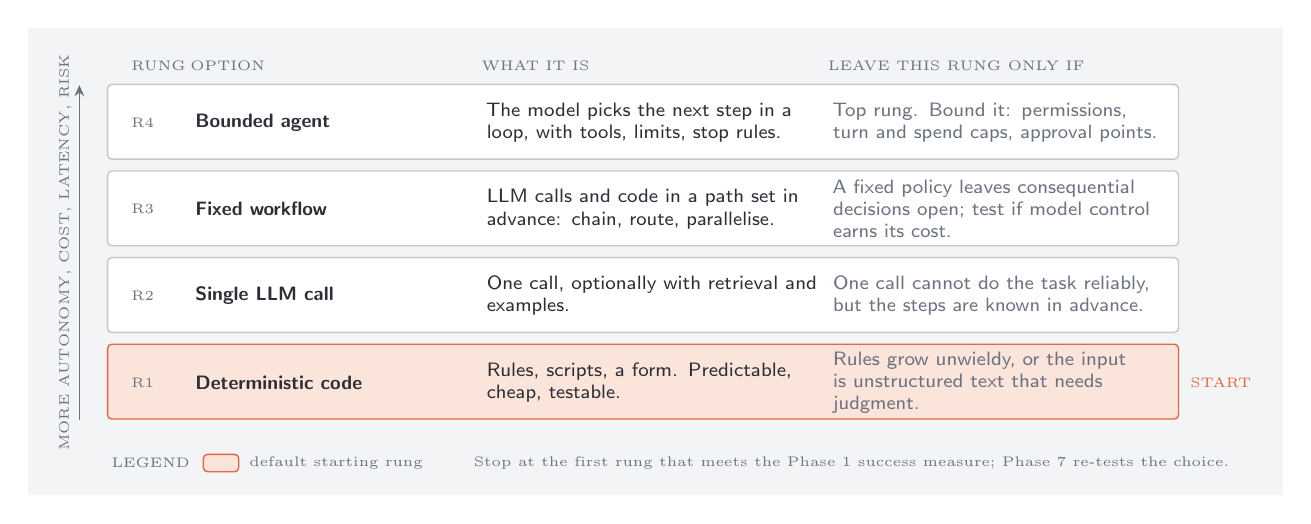
\begin{tikzpicture}[dp]
\def\rw{13.6}
\node[lab, anchor=west] at (0.25,4.5) {RUNG};
\node[lab, anchor=west] at (1.0,4.5) {OPTION};
\node[lab, anchor=west] at (4.7,4.5) {WHAT IT IS};
\node[lab, anchor=west] at (9.1,4.5) {LEAVE THIS RUNG ONLY IF};
\foreach \y/\st/\r/\name/\what/\leave in {
  0.0/focal/R1/Deterministic code/{Rules, scripts, a form. Predictable, cheap, testable.}/{Rules grow unwieldy, or the input is unstructured text that needs judgment.},
  1.1/box/R2/Single LLM call/{One call, optionally with retrieval and examples.}/{One call cannot do the task reliably, but the steps are known in advance.},
  2.2/box/R3/Fixed workflow/{LLM calls and code in a path set in advance: chain, route, parallelise.}/{A fixed policy leaves consequential decisions open; test if model control earns its cost.},
  3.3/box/R4/Bounded agent/{The model picks the next step in a loop, with tools, limits, stop rules.}/{Top rung. Bound it: permissions, turn and spend caps, approval points.}} {
  \node[\st, minimum width=\rw cm, minimum height=0.95cm, anchor=south west] at (0,\y) {};
  \node[lab, anchor=west] at (0.25,\y+0.475) {\r};
  \node[anchor=west, font=\sffamily\scriptsize\bfseries] at (1.0,\y+0.475) {\name};
  \node[anchor=west, text width=4.2cm, align=left] at (4.7,\y+0.475) {\what};
  \node[anchor=west, text width=4.15cm, align=left, text=dpmute] at (9.1,\y+0.475) {\leave};
}
\draw[->, draw=dpmute, line width=0.6pt] (-0.35,0) -- (-0.35,4.25)
  node[lab, midway, rotate=90, above=1pt] {MORE AUTONOMY, COST, LATENCY, RISK};
\node[lab, text=dpcoral, anchor=west] at (\rw+0.1,0.475) {START};
\begin{scope}[yshift=-0.55cm]
\node[lab, anchor=west] at (0,0) {LEGEND};
\node[focal, minimum width=0.45cm, minimum height=0.22cm, inner sep=0pt] at (1.45,0) {};
\node[lab, anchor=west] at (1.75,0) {default starting rung};
\node[lab, anchor=west] at (4.6,0) {Stop at the first rung that meets the Phase 1 success measure; Phase 7 re-tests the choice.};
\end{scope}
\end{tikzpicture}
\caption{The Phase~2 ladder. The exit conditions paraphrase Anthropic \cite[``When (and when not) to use agents'']{bea}, OpenAI \cite[pp.~5--6]{openai} and Northeastern \cite[slides~9, 10, 14]{neu4a}; arranging them as a ladder, and the tighter wording of the exit from the fixed workflow, are my synthesis \inferred.}
\label{fig:ladder}
\end{figure}

\textbf{Criteria for moving up.}
\begin{itemize}
\item Anthropic: find the simplest solution possible and add complexity only when it demonstrably improves results; workflows suit well-defined tasks, agents suit open-ended problems where the steps cannot be predicted, at the price of cost, latency and compounding errors \cite[``When (and when not) to use agents'']{bea}.
\item OpenAI: consider an agent when the task needs complex judgment, the rule set has become unwieldy, or it relies heavily on unstructured data; otherwise a deterministic solution may suffice \cite[pp.~5--6]{openai}.
\item Northeastern distinguishes fixed workflows and one-time routing from a loop in which the model selects actions using their results. Cycles alone are insufficient: the model must direct the next action \cite[slides~9, 10, 14]{neu4a}.
\item CMU places developer-defined workflows, plan-then-execute and adaptive agents on one spectrum: a fixed plan is faster, cheaper and more predictable, and replanning should be bought only when its feedback is worth the cost \cite[p.~16]{cmu5}.
\item Stanford CS146S, for skills: a single fixed command is a shell alias, not a skill; a skill needs repetition and a real decision point \cite[Part~I]{cs146s3}.
\end{itemize}

\textbf{Leaving the fixed workflow.} ``The steps cannot be predicted'' is not enough to leave the fixed-workflow rung, because a fixed workflow can branch, retry and escalate. Write the strongest fixed policy you can maintain, including those branches, and list the decisions it leaves unresolved. No branch may hide an agent: ``diagnose and repair'' is not a step unless the policy says how. Move up only if those unresolved decisions are worth more than the added cost and risk \inferred.

\textbf{Before authorizing a bounded agent,} answer three questions about feedback \inferred:
\begin{itemize}
\item What observation will guide the model's next decision during a run?
\item What checks success independently of the model, in a way the agent cannot alter?
\item How has that check been tested, for example on cases already known to be good and bad?
\end{itemize}
Weak or misleading feedback can misdirect the agent's adaptation. Record its limitations and test whether it is informative enough for the decisions the agent will make \inferred. The screening companion gives the cases behind these feedback questions and the exit from the fixed workflow \cite[Sections~3--4]{screen}.

\textbf{Gap in the courses.} In the public material checked, no course asks students to write down why a script or a single call would not do. Only the Anthropic and OpenAI guides state the test. This phase makes it an explicit gate. The decision is provisional: Phase~7 confirms it empirically by comparing against the simpler option, as CS329A HW3 does when it builds a single-call baseline before adding routing, decomposition and refinement \cite[Parts~0--3]{cs329a}, and as Mannheim does with a non-LLM baseline \cite[slide~26]{mannheim}.

\begin{gate}
The chosen option is recorded, with the evidence for rejecting each relevant simpler alternative and any remaining unknowns. If the provisional choice is a bounded agent, the record also holds the strongest maintainable fixed policy, the decisions it appears to leave unresolved, their expected value, the answers to the three feedback questions and the planned comparison.
\end{gate}

% ---------------------------------------------------------------------------
\phase{3}{Decompose the task and assign ownership}

\begin{goal}
Split the work into tasks and subtasks, and decide for each whether code, the model or a human owns it.
\end{goal}

\textbf{Allocation rules} (Northeastern, week~3b, rules~1--6 \cite{neu3b}; Figure~\ref{fig:owners}):
\begin{itemize}
\item Policy, calculations, permissions and budgets live in \textbf{code}; contextual judgment and tool selection live in the \textbf{model}. ``The model proposes; the runtime disposes.''
\item Prompt rules that read like code belong in code.
\item Tools validate their own inputs, obtain their own prerequisites, and return both facts and verdicts, so they cannot be talked out of a rule.
\end{itemize}

\begin{figure}[htbp]
\centering
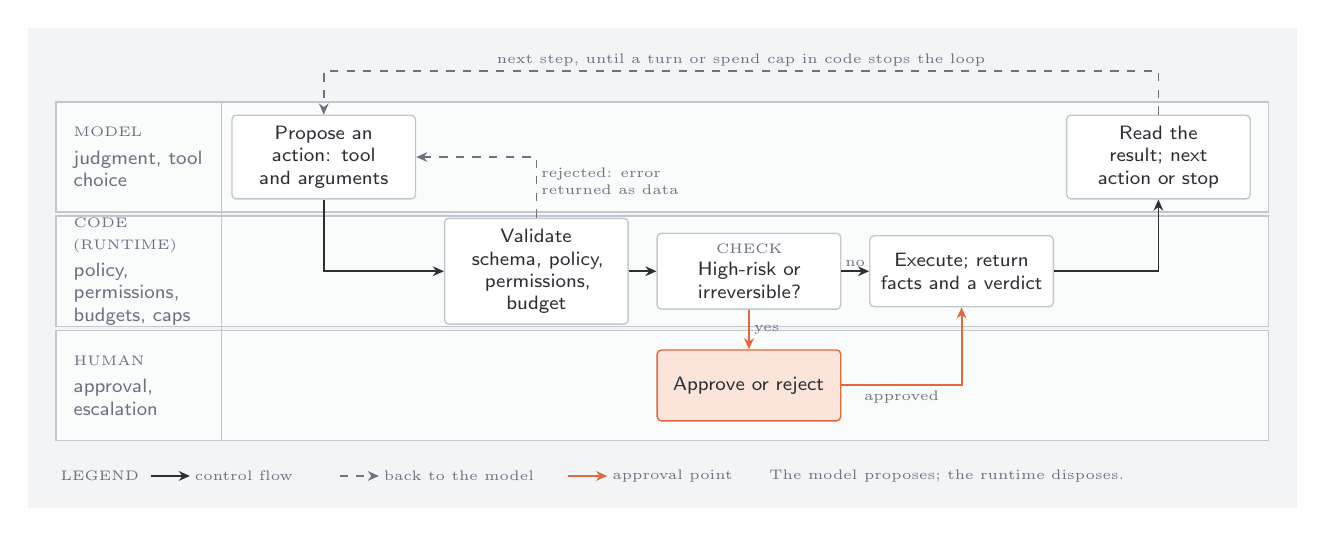
\begin{tikzpicture}[dp, card/.style={box, text width=2.05cm, minimum height=0.9cm}]
% lanes
\foreach \y/\t/\s in {2.9/MODEL/{judgment, tool choice}, 1.45/{CODE (RUNTIME)}/{policy, permissions, budgets, caps}, 0/HUMAN/{approval, escalation}} {
  \draw[dpline, line width=0.5pt, fill=white!60!dpbg] (0,\y-0.7) rectangle (15.4,\y+0.7);
  \node[anchor=west, align=left, text width=1.9cm] at (0.1,\y) {\dptag{\t}\\[2pt]{\color{dpmute}\s}};
}
\draw[dpline, line width=0.5pt] (2.1,-0.7) -- (2.1,3.6);
% steps
\node[card] (s1) at (3.4,2.9) {Propose an action: tool and arguments};
\node[card] (s2) at (6.1,1.45) {Validate schema, policy, permissions, budget};
\node[card] (s3) at (8.8,1.45) {\dptag{check}\\High-risk or irreversible?};
\node[card, focal] (s4) at (8.8,0) {Approve or reject};
\node[card] (s5) at (11.5,1.45) {Execute; return facts and a verdict};
\node[card] (s6) at (14.0,2.9) {Read the result; next action or stop};
% flow
\draw[flow] (s1.south) |- (s2.west);
\draw[flow] (s2) -- (s3);
\draw[hot] (s3) -- node[lab, right] {yes} (s4);
\draw[flow] (s3) -- node[lab, above] {no} (s5);
\draw[hot] (s4.east) -| node[lab, pos=0.25, below] {approved} (s5.south);
\draw[flow] (s5.east) -| (s6.south);
\draw[back] (s2.north) |- node[lab, pos=0.3, right, align=left] {rejected: error\\returned as data} (s1.east);
\draw[back] (s6.north) -- ++(0,0.55) -| node[lab, pos=0.25, above] {next step, until a turn or spend cap in code stops the loop} (s1.north);
% legend
\begin{scope}[yshift=-1.15cm]
\node[lab, anchor=west] at (0,0) {LEGEND};
\draw[flow] (1.2,0) -- ++(0.5,0) node[lab, right] {control flow};
\draw[back] (3.6,0) -- ++(0.5,0) node[lab, right] {back to the model};
\draw[hot] (6.5,0) -- ++(0.5,0) node[lab, right] {approval point};
\node[lab, anchor=west] at (9.0,0) {The model proposes; the runtime disposes.};
\end{scope}
\end{tikzpicture}
\caption{Ownership for one step of an agent loop: the model proposes, code validates and executes, and a human approves high-risk actions. Allocation follows Northeastern \cite[rules~1--6]{neu3b}; human intervention on high-risk actions follows OpenAI \cite[pp.~24--31]{openai}. The sequence is an illustration \inferred.}
\label{fig:owners}
\end{figure}

\textbf{Design checklist} (CMU lecture~5, p.~46 \cite{cmu5}):
\begin{itemize}
\item Are the subtasks really separable, and would different parts benefit from different models?
\item Which observations should change the plan?
\item How will errors and context be kept from piling up?
\item What information or authority must stay separate, and who approves irreversible actions?
\end{itemize}

\textbf{Also record:} stopping conditions (turn and spend caps), the points where a human must approve, and the escalation path when the agent is unsure. LangGraph's method maps the workflow into discrete steps and labels each as an LLM step, a data step, an action or a human-input step \cite[steps~1--2]{langgraph}. OpenAI requires human intervention on failure thresholds and high-risk actions \cite[pp.~24--31]{openai}.

\textbf{Single or multiple agents.} OpenAI recommends maximising a single agent first and considering a split when complex instructions or overlapping tools impair performance \cite[p.~16]{openai}. Anthropic describes additional patterns for parallel work and dynamic delegation \cite[``Parallelization'', ``Orchestrator-workers'']{bea}. Berkeley's Lab~2 recommends planning, generation and verification agents for its Lean task \cite{brkadv}; treat that as a design for that task, not a default.

\begin{gate}
A task map lists every subtask with its owner (code, model, human), the stopping conditions, and the approval points.
\end{gate}

% ---------------------------------------------------------------------------
\phase{4}{Define the evaluation}

\begin{goal}
Decide how success will be measured before building, so the prototype is judged against evidence rather than demos.
\end{goal}

\textbf{Contents}
\begin{itemize}
\item \textbf{A first test set.} Anthropic recommends starting early with 20--50 simple tasks drawn from real failures, because evals get harder to build the longer you wait \cite{anthevals}. Include known-good cases, known failures and edge cases. Berkeley requires test cases with known outcomes, including edge cases, and asks that a human be able to solve each task \cite[pp.~82--85, 91]{brkeval}. Those known-outcome cases test the evaluator itself \cite[p.~85]{brkeval}.
\item \textbf{Metrics} across quality, cost, latency and safety. Mannheim's method: define success criteria, choose the method (code checks, LLM judge, human review), use tooling, iterate \cite[p.~76]{mannheim4}. CMU evaluates at four levels: tool selection, arguments, trajectory and final task, plus efficiency, reliability and safety \cite[pp.~54--56]{cmu2}.
\item \textbf{Reliability, not only success rate.} Run each task several times to measure consistency; test robustness by injecting tool faults, changing tool-interface formats and paraphrasing prompts; and, if the agent reports confidence, measure its calibration. Rabanser et al.\ define such metrics in four groups (consistency, robustness, predictability, safety) and used five runs per task, a fault probability of 0.2 and five paraphrases \cite[\S3, Table~2; \S4.1]{reliab}. Five runs is their experimental setting, not a prescribed minimum; choose the count to balance estimation precision against cost \inferred.
\item \textbf{The grader.} Prefer code checks, then model graders, with humans to calibrate \cite{anthevals}. An LLM judge is not always needed: verifiable tasks can be checked objectively \cite[pp.~17, 71]{brkeval}.
\item \textbf{Development and held-out cases.} Use development cases for iteration and model selection, and keep held-out cases to check generalisation before release. Validate graders against known successes and failures, and reset environment and memory state between independent trials \cite[``Collaborating with agents'']{anthtools}\cite[steps~2, 4, 5]{anthevals}.
\item \textbf{The baseline}: the simpler rung from Phase~2, run on the same set.
\item \textbf{The release bar}: the threshold, on these metrics, that Phase~8 must confirm. For reliability, consider pass$^k$ (success on all $k$ attempts) rather than pass@$k$ \cite[p.~30]{brkdeploy}.
\end{itemize}

\textbf{Order dispute.} The Anthropic evals post and the Berkeley project put evaluation first (Berkeley's project structure introduces evaluator development as Phase~1 and participant-agent development as Phase~2 \cite[Grading, Project Timeline]{brkcourse}; both final submissions share a deadline, so this is an emphasis, not a strict gate); the Anthropic tools post prototypes first and then evaluates \cite{anthtools}; OpenAI sets up evals as the baseline for model selection \cite[p.~8]{openai}. Resolution \inferred: write a small set before building, then grow it from the failures found in Phase~7.

\begin{gate}
A versioned test set, the metrics, the grader for each, the baseline and the release bar are written down.
\end{gate}

% ---------------------------------------------------------------------------
\phase{5}{Design tools, state and context}

\begin{goal}
Specify everything the model can touch and see, so that its actions are constrained by design rather than by prompt wording.
\end{goal}

\textbf{Tools}
\begin{itemize}
\item Prefer a few workflow-level tools to many thin endpoint wrappers; namespace them; return high-signal, token-efficient results; make errors actionable \cite{anthtools}.
\item Put constraints in the schema (enums, ranges, required fields), shape the outputs, return errors as data, treat the docstring as the contract, and put a brake on write tools (read-only hints, dry runs) \cite[Part~II]{cs146s2}.
\item Design the interface to be hard to misuse (poka-yoke), for example requiring absolute paths \cite[Appendix~2]{bea}.
\item Call a tool only when its benefit outweighs its latency, cost, failure modes and risk \cite[p.~5]{cmu2}.
\end{itemize}

\textbf{State and context}
\begin{itemize}
\item Define the state the system carries between steps, how it changes, and what happens on each error path \cite[steps~3--4]{langgraph}.
\item Decide what context each step needs and keep it minimal and high-signal \cite{anthcontext}. Persistent memory is a design choice, not a required component.
\item For a recurring agent, track progress per source with a stored bookmark rather than a fixed time window. If a source cannot be read, keep its bookmark and say so in the output; never report it as ``nothing new'' \cite[Sources]{anthauto}.
\item Record a side effect as done only after the destination confirms it, and check for an existing result before retrying to reduce duplicate effects \cite[Destination]{anthauto}.
\item Keep the rules the agent must follow in a store it can read but not edit; have it re-read them every run and stop if it cannot \cite[Memory]{anthauto}.
\item Treat curated context as an owned asset. Notion separates data context (metrics, sources, required filters), business context and routing guidance, and assigns owners and review to keep them current \cite[``Connecting data and business context'', ``Keeping data and business context current'']{notion}.
\end{itemize}

\textbf{Permission boundaries.} Least privilege for every tool and credential, sandboxed execution, and paths confined to a working directory \cite{jhu}\cite{cmu13}. Minimal OAuth scopes, each with a stated reason \cite{cs146s2}. When the agent acts for a user, let it use that user's own credentials so existing access controls apply, and have it report denied access instead of working around it \cite[``Governing the agent and its data access'', ``Clear instructions for repeatable analysis'']{notion}.

\begin{gate}
Every tool has a contract (inputs, outputs, errors, side effects, permission level); the state model and error paths are written; permissions are listed.
\end{gate}

% ---------------------------------------------------------------------------
\phase{6}{Build a minimal prototype and select models}

\begin{goal}
Get one path working end to end with full tracing, then choose models by measuring them on the Phase~4 development set.
\end{goal}

\textbf{Build}
\begin{itemize}
\item Build the simplest version of the chosen rung. Anthropic suggests starting with direct API calls rather than a framework, so the mechanics stay visible \cite{bea}; Google calls a production-grade framework essential \cite[p.~23]{gintro}. Resolution \inferred: specify the capabilities you need and choose a library only if it supplies them.
\item Test each tool on its own before wiring it in, and write the system prompt last \cite{neudada}.
\item Trace every run: prompts, tool calls, results, cost and latency. Phase~7 depends on it.
\end{itemize}

\textbf{Select models}
\begin{itemize}
\item OpenAI: prototype with the most capable model to set a quality baseline, then try smaller models and keep them where they still meet the target \cite[p.~8]{openai}.
\item Mannheim recommends free-model prototyping, small-model main experiments, and selective use of stronger models after estimating cost \cite[slide~28]{mannheim}. CS329A recommends smaller, cost-effective models during development before scaling to larger models \cite[``API Configuration and Setup'']{cs329a}.
\item JHU A2 compares models empirically across languages and prompting strategies \cite{jhua2}.
\item Resolution \inferred: these optimise different budgets. If quality is uncertain, start strong to learn what is achievable; if spend is the binding constraint, start cheap and escalate. In both cases compare on the Phase~4 development set, and record quality, cost and latency per model.
\end{itemize}

\begin{gate}
One traced path runs end to end, and a model table (quality, cost, latency on the development set) supports the chosen model or models.
\end{gate}

% ---------------------------------------------------------------------------
\phase{7}{Evaluate, diagnose and iterate}

\begin{goal}
Find out why the system fails, fix the causes, and confirm that the added complexity earns its cost.
\end{goal}

\textbf{The loop} (CS329T HW1, the course's ``standard iterative process'' \cite[\S\S1--2]{cs329t}; Figure~\ref{fig:loop}):
\begin{enumerate}
\item Run the system on the development set and read the traces.
\item Label failures by hand, grouped into error classes.
\item If you use LLM judges, check them against your hand labels before trusting them.
\item Change prompts, tools or architecture and rerun.
\end{enumerate}

\begin{figure}[htbp]
\centering
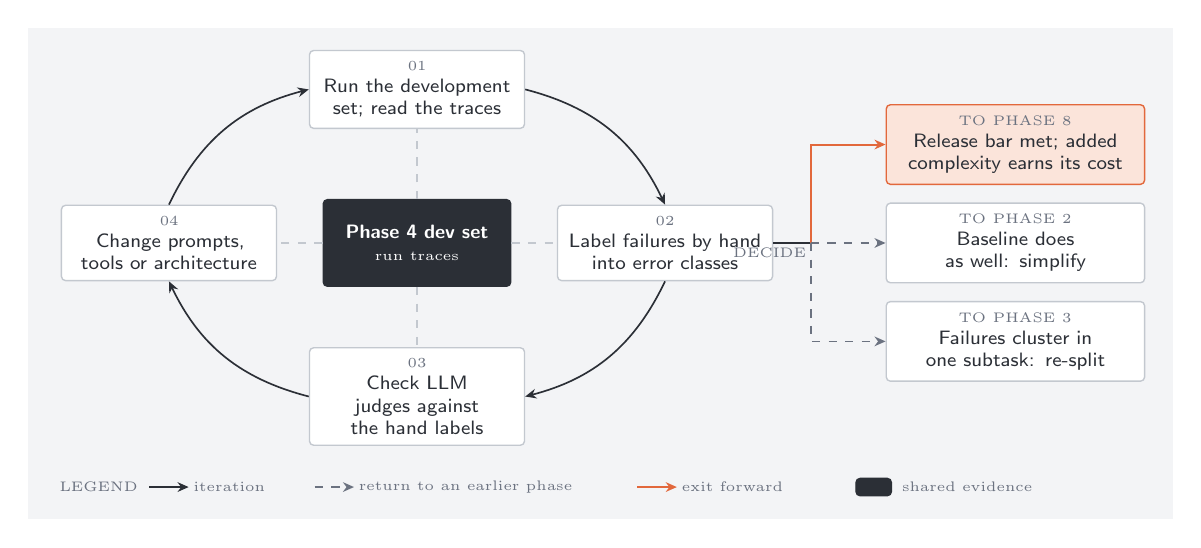
\begin{tikzpicture}[dp, card/.style={box, text width=2.45cm, minimum height=0.95cm}]
\node[hub, text width=2.1cm, minimum height=1.1cm] (hub) at (0,0) {\textbf{Phase 4 dev set}\\{\dpmono\tiny run traces}};
\node[card] (n) at (0,1.95) {\dptag{01}\\Run the development set; read the traces};
\node[card] (e) at (3.15,0) {\dptag{02}\\Label failures by hand into error classes};
\node[card] (s) at (0,-1.95) {\dptag{03}\\Check LLM judges against the hand labels};
\node[card] (w) at (-3.15,0) {\dptag{04}\\Change prompts, tools or architecture};
\draw[flow] (n.east) to[bend left=25] (e.north);
\draw[flow] (e.south) to[bend left=25] (s.east);
\draw[flow] (s.west) to[bend left=25] (w.south);
\draw[flow] (w.north) to[bend left=25] (n.west);
\draw[dpline, dashed, line width=0.5pt] (hub.north) -- (n.south) (hub.east) -- (e.west) (hub.south) -- (s.north) (hub.west) -- (w.east);
% exits
\node[card, focal, text width=3.0cm] (x8) at (7.6,1.25) {\dptag{to phase 8}\\Release bar met; added complexity earns its cost};
\node[card, text width=3.0cm] (x2) at (7.6,0) {\dptag{to phase 2}\\Baseline does as well: simplify};
\node[card, text width=3.0cm] (x3) at (7.6,-1.25) {\dptag{to phase 3}\\Failures cluster in one subtask: re-split};
\coordinate (d) at (5.0,0);
\draw[dpink, line width=0.6pt] (e.east) -- (d);
\draw[hot] (d) |- (x8.west);
\draw[back] (d) -- (x2.west);
\draw[back] (d) |- (x3.west);
\node[lab, below left] at (d) {DECIDE};
% legend
\begin{scope}[yshift=-3.1cm, xshift=-4.6cm]
\node[lab, anchor=west] at (0,0) {LEGEND};
\draw[flow] (1.2,0) -- ++(0.5,0) node[lab, right] {iteration};
\draw[back] (3.3,0) -- ++(0.5,0) node[lab, right] {return to an earlier phase};
\draw[hot] (7.4,0) -- ++(0.5,0) node[lab, right] {exit forward};
\node[hub, minimum width=0.45cm, minimum height=0.22cm, inner sep=0pt] at (10.4,0) {};
\node[lab, anchor=west] at (10.7,0) {shared evidence};
\end{scope}
\end{tikzpicture}
\caption{The Phase~7 loop. Steps 01--04 follow CS329T HW1 \cite[\S\S1--2]{cs329t} and Mannheim \cite[slide~26]{mannheim}; the exits and their conditions are my synthesis \inferred.}
\label{fig:loop}
\end{figure}

\textbf{Supporting practice}
\begin{itemize}
\item Mannheim: define error classes by hand on a sample, count them, then automate the analysis \cite[slide~26]{mannheim}.
\item CS329T's Agent GPA checks goal fulfilment, plan quality, plan adherence, tool selection, tool calling, execution efficiency and logical consistency \cite[slide~21]{cs329tl3}.
\item Google: evaluate end-to-end outcomes first, then inspect trajectories to diagnose \cite[pp.~17--19]{gquality}. Chip Huyen catalogues planning and tool failure modes and recommends testing tools independently \cite{huyen}.
\item Separate capability evals (can it do this?) from regression evals (did a change break it?) \cite{anthevals}.
\item A run without errors does not establish that its answer is correct. Notion found that a query could run cleanly and still answer the wrong question, with the meaning, routing, measurement or interpretation wrong, and that more retrieval or retries did not automatically help \cite[``Why working SQL isn't enough'', ``Seeing what the agent actually did'']{notion}.
\end{itemize}

\textbf{When Phase~2 chose a bounded agent,} the baseline is the strongest fixed workflow, and the comparison is the matched one planned on the screening worksheet: the same model, starting information, tools, check and limits in both arms, on cases used to design neither, so that the only difference is who selects the next step \cite[Section~4]{screen}.

\textbf{Return paths.} If the system does not beat the Phase~2 baseline by enough to justify its cost and latency, go back to Phase~2 and simplify. If failures cluster in one subtask, revisit its ownership in Phase~3 \inferred.

\begin{gate}
Error classes and counts are recorded, graders are validated, and the selected design meets the agreed success and safety thresholds. Any added complexity has a measured benefit that justifies its cost and latency; otherwise simplify and re-evaluate \inferred.
\end{gate}

% ---------------------------------------------------------------------------
\phase{8}{Harden safety and approve release}

\begin{goal}
Show that the boundaries from Phases 3 and 5 hold under attack and misuse, and that the release bar is met.
\end{goal}

\begin{itemize}
\item Run adversarial and misuse cases: prompt injection through tool outputs and retrieved content, attempts to exceed permissions, and inputs that should be refused. Buffalo's Lab~5 asks where autonomy helps and where it should be restricted \cite{buffalo}; CMU covers sandboxing and approval points \cite{cmu13}.
\item Layer guardrails: LLM-based checks, rules and moderation, added as edge cases appear; route high-risk actions and repeated failures to a human \cite[pp.~24--31]{openai}. Guardrails can run as separate parallel calls \cite{bea}.
\item Guardrails can miss attacks; Mannheim's safety deck covers their limits \cite[pp.~17--23]{mannheim8}. Measure their effectiveness against the system's threat model, rely on enforced permission boundaries, and explicitly assess residual risk \inferred.
\item Production concerns listed by Sierra: guardrails and enforced determinism, regression testing, user simulation, staging and release, model migration and failover \cite[p.~10]{brkdeploy}.
\item Treat safety results as hard constraints: report them separately instead of averaging them into an overall score \cite[\S3.5]{reliab}. Where the agent's output is the final action, with no human review, set a higher reliability bar than for an assistant \cite[\S5, Recommendation~4]{reliab}.
\item For agents that run unattended, use read-only credentials wherever the agent only reads, and cap what each run can spend. Anthropic suggests starting the cap at three to five times the cost of a normal run and tightening it from real numbers \cite[Guardrails]{anthauto}.
\item Confirm the Phase~4 release bar, including the held-out generalisation check and regression and safety evaluations, and record who signed off. Google describes evaluation gates before release, including a manual gate for less mature teams \cite[pp.~12, 17--18]{gprod}.
\end{itemize}

\begin{gate}
Adversarial results are recorded, every unacceptable failure from Phase~1 has a tested control, and the release bar is met and signed off.
\end{gate}

% ---------------------------------------------------------------------------
\phase{9}{Deploy gradually and maintain}

\begin{goal}
Release in stages with a way back, watch the system in use, and turn what you learn into tests.
\end{goal}

\begin{itemize}
\item Version prompts, tools, models and the test set together. Roll out in stages with a rollback path \cite[pp.~15--16, 24]{gprod}.
\item Monitor quality, cost, latency and safety events in production. Monitoring complements evals; it does not replace them \cite{anthevals}.
\item Triage production failures and add representative regression cases to the Phase~4 set \cite[p.~24]{gprod}.
\item Re-run the full evaluation on any model change \cite[p.~18]{gprod}. Sierra's development cycle is build, test, optimise, repeated \cite[p.~17]{brkdeploy}.
\item Re-evaluate at regular intervals, not only after changes. Rabanser et al.\ call for periodic evaluation on evolving benchmarks, so that reliability that degrades silently is caught \cite[\S5 and App.~A, Recommendation~1]{reliab}. In deployment, apply this by regularly re-evaluating against cases and environments updated to reflect current conditions \inferred.
\item Start small and validate with real users \cite[conclusion]{openai}. For a scheduled agent, trigger a run by hand before relying on the schedule \cite[Schedule]{anthauto}.
\item Review production traces on a schedule. At Notion, a nightly review agent records missing, stale or conflicting context, and a separate triage agent applies authorised fixes and sends ambiguous or higher-risk changes to a person; it notes that query success and rising usage are useful signals, but ``neither proves accuracy'' \cite[``Keeping data and business context current'', ``Seeing what the agent actually did'']{notion}.
\end{itemize}

\begin{gate}
The system is versioned, the rollout and rollback plan is tested, monitoring is live, and there is a routine for moving production failures into the test set.
\end{gate}

% ---------------------------------------------------------------------------
\section*{Different emphases and my design choices}
\addcontentsline{toc}{section}{Different emphases and my design choices}

\begin{center}
\small
\begin{tabularx}{\linewidth}{@{}p{2.8cm} L L@{}}
\toprule
Question & Positions & How this process treats it \\
\midrule
Model order & Strongest first, then downsize \cite{openai}; cheap first, then escalate \cite{mannheim,cs329a} & Choose by budget; always compare on the development set (Phase~6) \\
Evals or prototype first & Evals early \cite{anthevals}; evaluator-first project structure \cite[Grading, Project Timeline]{brkcourse}; prototype then evaluate \cite{anthtools} & Small set before building, grown from failures (Phase~4) \\
One agent or several & Single agent first \cite[p.~16]{openai}; three agents for a Lean task \cite{brkadv} & Start simple; add agents when measured benefits justify the coordination cost \inferred{} (Phase~3) \\
Frameworks & Direct API calls first \cite{bea}; framework essential \cite{gintro} & Specify capabilities, not a library (Phase~6) \\
LLM judges & Common in course rubrics \cite{cs329t}; objective checks for verifiable tasks \cite{brkeval} & Code checks first; validate judges against humans (Phases 4, 7) \\
Research framing & Mechanism $\rightarrow$ manipulation $\rightarrow$ measured behaviour \cite{neuresearch} & Research novelty is not a product requirement; mechanism-based experiments can still test design choices \inferred \\
\bottomrule
\end{tabularx}
\end{center}

\section*{Limits of this document}
\addcontentsline{toc}{section}{Limits of this document}

\begin{itemize}
\item The evidence is the public material checked on 9 October 2026. Unpublished rubrics (CMU's project, Buffalo, Stanford CS146S's final project), JHU lecture PDFs over 10\,MB, Google Slides and PPTX decks, and lecture videos were not read. ``Not found'' means not found in that material.
\item The Anthropic, OpenAI and Google guides were read through extracted text and summaries; page and section numbers come from those reads. The reliability paper \cite{reliab} was read in its arXiv HTML version (v3). The two practitioner posts \cite{anthauto,notion} each describe one system; Notion's outcome figures are self-reported.
\item The phase order, the Phase~2 ladder, the gates and the resolutions of disagreements are my synthesis.
\end{itemize}

\section*{Authorship and use of AI tools}
\addcontentsline{toc}{section}{Authorship and use of AI tools}

I am the sole author. I used AI tools in preparing this document and disclose their role here.
\emph{Claude} (Anthropic, through Claude Code) read the course materials and practitioner guides, and drafted and revised the text and diagrams under my direction.
\emph{Codex} (OpenAI) made an independent pass over the same sources and reviewed the citations; its corrections were applied.
Claude also drafted the appendix examples and their diagrams under my direction, and Codex reviewed them against the phases and the screening worksheet.
Words taken from a source are in quotation marks with the source. Practices taken from a source are cited to it, with a page or section reference where one is available. Statements marked \inferred{} are my own synthesis.
I set the questions, decided what to include and am responsible for the content.

% ---------------------------------------------------------------------------
\section*{Appendix: Worked examples}\label{app:examples}
\addcontentsline{toc}{section}{Appendix: Worked examples}

Three examples follow. Each takes one task through the process:
\begin{itemize}
\item the Phase~1 brief;
\item the screening worksheet that feeds Phase~2 \cite[Section~6]{screen};
\item the decisions recorded in the later phases.
\end{itemize}
A diagram in each example shows where the model chooses the next step, and where code and people keep control.
In all three, the strongest fixed workflow is built first. A bounded agent is kept only for the decision that the fixed workflow leaves open, and only if it wins the Phase~7 comparison.
Two rules hold in every example and are not repeated in the tables. The acceptance check sits with code or a person, outside the model's control (row A3). Phase~8 ends, as in the main text, with the release bar confirmed and the release signed off.
The examples are illustrations, not reports of built systems \inferred.

% lanes for the example diagrams: model, code (runtime), human
\newcommand{\exlanes}{%
  \foreach \y/\t/\s in {2.9/MODEL/{chooses the next step}, 1.45/{CODE (RUNTIME)}/{rules, limits, tools}, 0/HUMAN/{approval, review}} {
    \draw[dpline, line width=0.5pt, fill=white!60!dpbg] (0,\y-0.7) rectangle (15.4,\y+0.7);
    \node[anchor=west, align=left, text width=1.9cm] at (0.1,\y) {\dptag{\t}\\[2pt]{\color{dpmute}\s}};
  }
  \draw[dpline, line width=0.5pt] (2.1,-0.7) -- (2.1,3.6);}

% ---------------------------------------------------------------------------
\clearpage
\subsection*{Example 1: a phone agent that acts during a call}

A small business wants its phone answered. The agent answers questions, books, moves or cancels appointments, writes a note to the CRM, and transfers the caller when it should.

\begin{center}
\makeatletter\def\@captype{figure}\makeatother
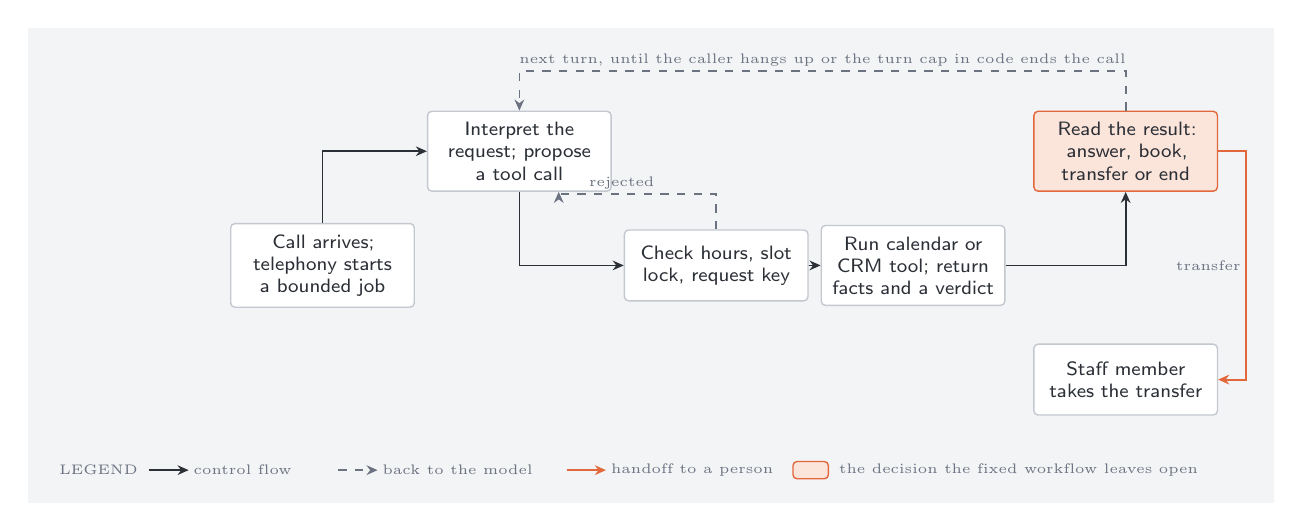
\begin{tikzpicture}[dp, card/.style={box, text width=2.05cm, minimum height=0.9cm}]
\exlanes
\node[card] (c1) at (3.4,1.45) {Call arrives; telephony starts a bounded job};
\node[card] (m1) at (5.9,2.9) {Interpret the request; propose a tool call};
\node[card] (c2) at (8.4,1.45) {Check hours, slot lock, request key};
\node[card] (c3) at (10.9,1.45) {Run calendar or CRM tool; return facts and a verdict};
\node[card, focal] (m2) at (13.6,2.9) {Read the result: answer, book, transfer or end};
\node[card] (h1) at (13.6,0) {Staff member takes the transfer};
\draw[flow] (c1.north) |- (m1.west);
\draw[flow] (m1.south) |- (c2.west);
\draw[flow] (c2) -- (c3);
\draw[flow] (c3.east) -| (m2.south);
\draw[hot] (m2.east) -- ++(0.35,0) |- node[lab, pos=0.25, left] {transfer} (h1.east);
\draw[back] (m2.north) -- ++(0,0.5) -| node[lab, pos=0.25, above] {next turn, until the caller hangs up or the turn cap in code ends the call} (m1.north);
\draw[back] (c2.north) -- ++(0,0.45) -| node[lab, pos=0.3, above] {rejected} ([xshift=0.5cm]m1.south);
\begin{scope}[yshift=-1.15cm]
\node[lab, anchor=west] at (0,0) {LEGEND};
\draw[flow] (1.2,0) -- ++(0.5,0) node[lab, right] {control flow};
\draw[back] (3.6,0) -- ++(0.5,0) node[lab, right] {back to the model};
\draw[hot] (6.5,0) -- ++(0.5,0) node[lab, right] {handoff to a person};
\node[focal, minimum width=0.45cm, minimum height=0.22cm, inner sep=0pt] at (9.6,0) {};
\node[lab, anchor=west] at (9.9,0) {the decision the fixed workflow leaves open};
\end{scope}
\end{tikzpicture}
\caption{Example~1. Code notices the call and enforces every booking rule; the model chooses the next tool call within the call; a person takes transfers. The arrangement is an illustration \inferred.}
\label{fig:ex1}
\end{center}

\begin{center}
\small
\begin{tabularx}{\linewidth}{@{}p{2.7cm} L@{}}
\toprule
Step & Decision \\
\midrule
Phase~1 brief & Success is the right outcome for each call, within a response-time limit. The unacceptable failures are a double booking and an action the caller did not ask for. \\
Row S & Always on. The telephony service notices the call, and each call is a bounded job that ends when the caller hangs up. \\
Rows 0a, 0b & A keypad menu with a booking link serves callers who know what they want. One call with calendar context handles simple requests. Test both first. \\
Rows A1--A3 & \textbf{Connecting step:} understanding what the caller wants. \textbf{Tools:} the calendar, the CRM, a knowledge base and call transfer. \textbf{Check:} each booking is compared with the caller's scripted intent, with zero duplicates, and the check is tried on known-good and known-bad calls. \\
Rows B1--B3 & \textbf{Fixed policy:} a dialogue state machine with multiple intents, corrections, retries and transfer. \textbf{Open decision:} a request that changes mid-call and conflicts with what the calendar returns. \textbf{Worth testing} only if such calls cost more than the agent adds in running and oversight. \\
Phase~2 choice & The state machine first. Add a bounded agent for the open decision only if rows B1--B3 hold. \\
Phase~3 & Code owns business hours, booking rules and the turn cap. The model proposes the next tool call. A person takes transfers (Figure~\ref{fig:ex1}). \\
Phase~4 & Simulated callers for each type of request. Measure the outcome per call and the latency per turn. Report duplicate bookings separately, as a safety result. \\
Phase~5 & Repeating a request cannot create a second booking; it returns the recorded outcome. The calendar locks each slot. Tools return facts and a verdict. \\
Phase~6 & A traced prototype on scripted calls. Choose the model by latency per turn as well as by outcome. \\
Phase~7 (row B4) & The state machine against the agent, with the same model, information, tools, check and limits, on callers used to design neither. \\
Phase~8 & Callers who try to talk the agent out of a rule. \\
Phase~9 & One business first. Review calls on a schedule, and turn failed calls into test cases. \\
\bottomrule
\end{tabularx}
\end{center}

% ---------------------------------------------------------------------------
\clearpage
\subsection*{Example 2: an investigation agent that resolves conflicting evidence}

Given a list of companies, the system finds each one's owner and cites its sources. Most entities resolve from a registry. The hard cases are renamed companies, subsidiaries and records that disagree.

\begin{center}
\makeatletter\def\@captype{figure}\makeatother
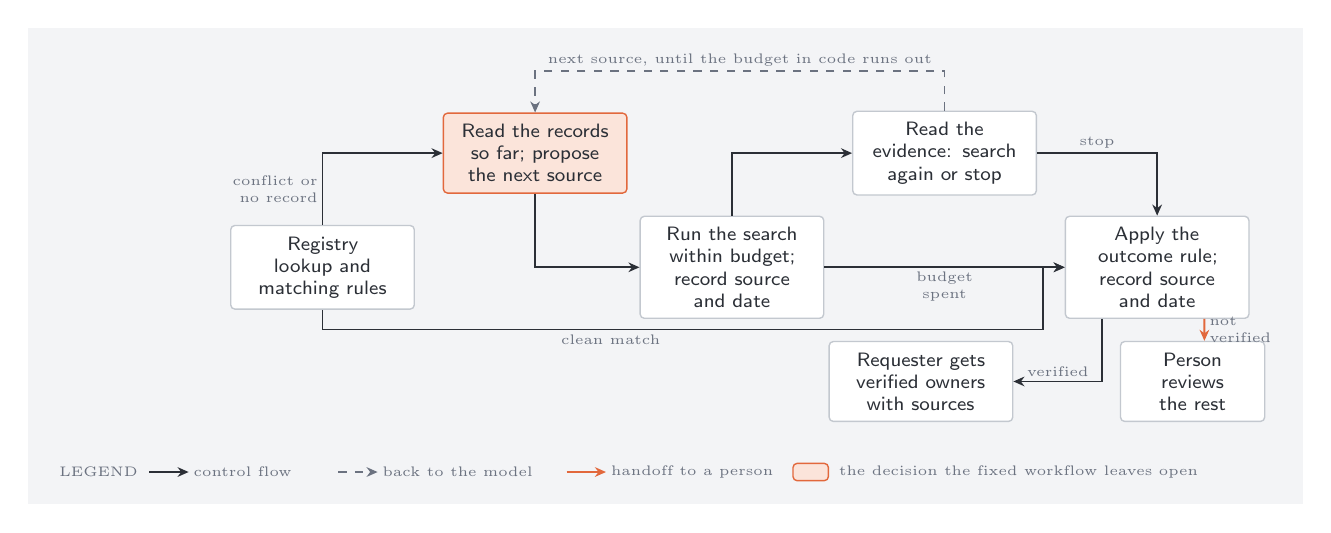
\begin{tikzpicture}[dp, card/.style={box, text width=2.05cm, minimum height=0.9cm}]
\exlanes
\node[card] (c1) at (3.4,1.45) {Registry lookup and matching rules};
\node[card, focal] (m1) at (6.1,2.9) {Read the records so far; propose the next source};
\node[card] (c2) at (8.6,1.45) {Run the search within budget; record source and date};
\node[card] (m2) at (11.3,2.9) {Read the evidence: search again or stop};
\node[card] (c3) at (14.0,1.45) {Apply the outcome rule; record source and date};
\node[card] (d1) at (11.0,0) {Requester gets verified owners with sources};
\node[card, text width=1.55cm] (h1) at (14.45,0) {Person reviews the rest};
\draw[flow] (c1.north) |- node[lab, pos=0.25, left, align=right] {conflict or\\no record} (m1.west);
\draw[flow] (m1.south) |- (c2.west);
\draw[flow] (c2.north) |- (m2.west);
\draw[flow] (c2.east) -- node[lab, below, align=center] {budget\\spent} (c3.west);
\draw[flow] (m2.east) -| node[lab, pos=0.25, above] {stop} (c3.north);
\draw[flow] (c1.south) -- ++(0,-0.25) -| node[lab, pos=0.2, below] {clean match} (12.55,1.45) -- (c3.west);
\draw[flow] ([xshift=-0.7cm]c3.south) |- node[lab, pos=0.75, above] {verified} (d1.east);
\draw[hot] ([xshift=0.6cm]c3.south) -- node[lab, right, align=left] {not\\verified} ([xshift=0.15cm]h1.north);
\draw[back] (m2.north) -- ++(0,0.5) -| node[lab, pos=0.25, above] {next source, until the budget in code runs out} (m1.north);
\begin{scope}[yshift=-1.15cm]
\node[lab, anchor=west] at (0,0) {LEGEND};
\draw[flow] (1.2,0) -- ++(0.5,0) node[lab, right] {control flow};
\draw[back] (3.6,0) -- ++(0.5,0) node[lab, right] {back to the model};
\draw[hot] (6.5,0) -- ++(0.5,0) node[lab, right] {handoff to a person};
\node[focal, minimum width=0.45cm, minimum height=0.22cm, inner sep=0pt] at (9.6,0) {};
\node[lab, anchor=west] at (9.9,0) {the decision the fixed workflow leaves open};
\end{scope}
\end{tikzpicture}
\caption{Example~2. Code resolves clean matches, stops the search when the budget is spent and applies the outcome rule. The model chooses where to look next only when the registry gives no clean match. A person reviews every outcome that is not verified. The arrangement is an illustration \inferred.}
\label{fig:ex2}
\end{center}

\begin{center}
\small
\begin{tabularx}{\linewidth}{@{}p{2.7cm} L@{}}
\toprule
Step & Decision \\
\midrule
Phase~1 brief & ``Owner'' is defined (legal, beneficial or ultimate parent) and dated. Success is a correct, sourced owner, or an honest ``unresolved''. The unacceptable failure is a confident wrong owner. \\
Row S & On demand. A list is handed over, and the job ends when every entity has an outcome. \\
Rows 0a, 0b & Registry lookups with matching rules resolve the clean cases. One call with search is the second baseline. \\
Rows A1--A3 & \textbf{Connecting step:} deciding which conflicting record to trust and where to look next. \textbf{Tools:} registries, web search and a browser, all read-only. \textbf{Check:} a reference set of entities with verified owners, plus cases that should end ``unresolved''. The check is tried on known-good and known-bad outputs. Agreement between sources guides a run but does not prove the answer. \\
Rows B1--B3 & \textbf{Fixed policy:} the registry, then a second source, then templated searches, then review. \textbf{Open decision:} which source to try when the registry gives no clean match. \textbf{Worth testing} only if the value of the cases it resolves, rare costly ones included, exceeds the agent's added model, search, oversight and failure costs. \\
Phase~2 choice & The fixed workflow first. Add a bounded agent for the hard cases only if rows B1--B3 hold. \\
Phase~3 & The model proposes the next source and how to read it. Code applies the outcome rule. \emph{Verified} needs two independent primary sources, such as a registry filing and a document not copied from it, that agree on the entity, the definition of owner and the date; a page that repeats another source does not count. The other outcomes are \emph{insufficient evidence}, \emph{conflict} and \emph{budget spent}, and a person reviews all three (Figure~\ref{fig:ex2}). \\
Phase~4 & Accuracy against known owners, the unresolved rate and the cost per entity. \\
Phase~5 & Every result carries its source and retrieval date, and each search counts against the budget. \\
Phase~6 & A traced prototype of the fixed workflow on a few known entities. Choose the smallest model that reads the records correctly. \\
Phase~7 (row B4) & The fixed workflow, with its branches and retries, against the agent. Both get the same model, information, tools and check, and the same limits on searches, model calls, time and total cost, on reference cases used to design neither. A run without errors can still name the wrong owner, so read the traces. \\
Phase~8 & Pages that carry injected instructions. \\
Phase~9 & Monitor the unresolved rate and the cost per entity, and add reviewed cases to the reference set. \\
\bottomrule
\end{tabularx}
\end{center}

% ---------------------------------------------------------------------------
\clearpage
\subsection*{Example 3: a planning run that adapts from performance data}

Each week the system proposes what content to make next, from the business's own material and last period's results. A fixed workflow then produces each approved item. The candidate agent is the planning run: within it, the model chooses which analysis to run next before it proposes the slate.

\begin{center}
\makeatletter\def\@captype{figure}\makeatother
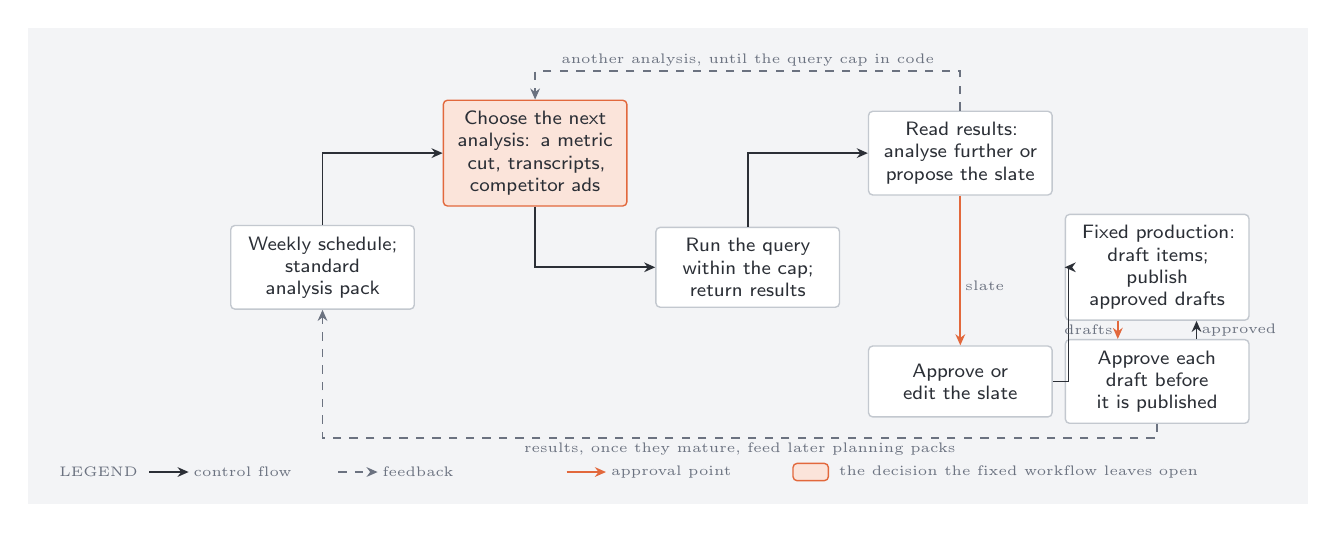
\begin{tikzpicture}[dp, card/.style={box, text width=2.05cm, minimum height=0.9cm}]
\exlanes
\node[card] (c1) at (3.4,1.45) {Weekly schedule; standard analysis pack};
\node[card, focal] (m1) at (6.1,2.9) {Choose the next analysis: a metric cut, transcripts, competitor ads};
\node[card] (c2) at (8.8,1.45) {Run the query within the cap; return results};
\node[card] (m2) at (11.5,2.9) {Read results: analyse further or propose the slate};
\node[card] (h1) at (11.5,0) {Approve or edit the slate};
\node[card] (c3) at (14.0,1.45) {Fixed production: draft items; publish approved drafts};
\node[card] (h2) at (14.0,0) {Approve each draft before it is published};
\draw[flow] (c1.north) |- (m1.west);
\draw[flow] (m1.south) |- (c2.west);
\draw[flow] (c2.north) |- (m2.west);
\draw[hot] (m2.south) -- node[lab, right, pos=0.6] {slate} (h1.north);
\draw[flow] (h1.east) -- ++(0.2,0) |- (c3.west);
\draw[hot] ([xshift=-0.5cm]c3.south) -- node[lab, left] {drafts} ([xshift=-0.5cm]h2.north);
\draw[flow] ([xshift=0.5cm]h2.north) -- node[lab, right] {approved} ([xshift=0.5cm]c3.south);
\draw[back] (m2.north) -- ++(0,0.5) -| node[lab, pos=0.25, above] {another analysis, until the query cap in code} (m1.north);
\draw[back] (h2.south) -- ++(0,-0.18) -| node[lab, pos=0.25, below] {results, once they mature, feed later planning packs} (c1.south);
\begin{scope}[yshift=-1.15cm]
\node[lab, anchor=west] at (0,0) {LEGEND};
\draw[flow] (1.2,0) -- ++(0.5,0) node[lab, right] {control flow};
\draw[back] (3.6,0) -- ++(0.5,0) node[lab, right] {feedback};
\draw[hot] (6.5,0) -- ++(0.5,0) node[lab, right] {approval point};
\node[focal, minimum width=0.45cm, minimum height=0.22cm, inner sep=0pt] at (9.6,0) {};
\node[lab, anchor=west] at (9.9,0) {the decision the fixed workflow leaves open};
\end{scope}
\end{tikzpicture}
\caption{Example~3. The agent sits inside one step of a fixed weekly workflow. Within the planning run it chooses the next analysis. A person approves the slate and then each draft; production stays fixed. Results mature weeks later and inform later runs, not the current one. The arrangement is an illustration \inferred.}
\label{fig:ex3}
\end{center}

\begin{center}
\small
\begin{tabularx}{\linewidth}{@{}p{2.7cm} L@{}}
\toprule
Step & Decision \\
\midrule
Phase~1 brief & Success is a slate the owner approves, and leads that grow over the quarter. The unacceptable failures are publishing without approval and false claims. \\
Row S & Always on, on a schedule. Code starts a weekly planning job that ends with a proposed slate. \\
Rows 0a, 0b & A rule (``more of what performed best'') and a multi-armed bandit over topics. One call given the standard analysis pack. \\
Rows A1--A3 & \textbf{Connecting step:} working out why something performed and choosing the next angle. \textbf{Tools:} analytics queries, transcript search and competitor-ad search. \textbf{Check:} within the run, query results; after it, approval of the slate and leads weeks later. The approval is tried on slates already known to be good and bad. \\
Rows B1--B3 & \textbf{Fixed policy:} the analysis pack plus drill-downs triggered by set anomalies. \textbf{Open decision:} which further analysis would explain a result the drill-downs do not. \textbf{Worth testing} only if the expected gain in leads exceeds the agent's added running, oversight and failure costs, and there is enough history to estimate that gain. \\
Phase~2 choice & A fixed workflow for production, and the bandit or one call for planning. Add a bounded agent for the planning run only if rows B1--B3 hold. Phase~2 warns that weak feedback can misdirect adaptation. \\
Phase~3 & A person approves the slate, and each draft before it is published. Code caps queries and spend per run (Figure~\ref{fig:ex3}). \\
Phase~4 & A factual check on drafts and the approval rate of slates before launch, then leads, reported with their delay. \\
Phase~5 & Read-only analytics access for planning; publishing tools only in the production workflow. \\
Phase~6 & A traced prototype of one planning run on past weeks. Choose the smallest model whose slates pass approval. \\
Phase~7 (row B4) & The fixed policy, with its drill-downs, against the agent. Both get the same model, information, tools, check and limits, on weeks used to design neither. Exposure is comparable, leads are measured over the same window, differences between weeks and channels are controlled, and the precision is estimated before the lead comparison is read. \\
Phase~8 & Injected text in transcripts and competitor pages. \\
Phase~9 & Watch for the loop chasing views at the expense of leads, and re-evaluate on a schedule. \\
\bottomrule
\end{tabularx}
\end{center}

% ---------------------------------------------------------------------------
\begin{thebibliography}{99}
\addcontentsline{toc}{section}{Sources}
\small

\bibitem{bea} Anthropic, ``Building Effective Agents''. \url{https://www.anthropic.com/engineering/building-effective-agents}
\bibitem{anthtools} Anthropic, ``Writing effective tools for agents''. \url{https://www.anthropic.com/engineering/writing-tools-for-agents}
\bibitem{anthevals} Anthropic, ``Demystifying evals for AI agents'' (Jan 2026). \url{https://www.anthropic.com/engineering/demystifying-evals-for-ai-agents}
\bibitem{anthcontext} Anthropic, ``Effective context engineering for AI agents''. \url{https://www.anthropic.com/engineering/effective-context-engineering-for-ai-agents}
\bibitem{openai} OpenAI, ``A practical guide to building agents''. \url{https://cdn.openai.com/business-guides-and-resources/a-practical-guide-to-building-agents.pdf}
\bibitem{gintro} Google/Kaggle, ``Introduction to Agents'' (May 2026). \url{https://www.kaggle.com/whitepaper-introduction-to-agents}
\bibitem{gquality} Google/Kaggle, ``Agent Quality'' (May 2026). \url{https://www.kaggle.com/whitepaper-agent-quality}
\bibitem{gprod} Google/Kaggle, ``Prototype to Production'' (May 2026). \url{https://www.kaggle.com/whitepaper-prototype-to-production}
\bibitem{langgraph} LangChain, ``Thinking in LangGraph''. \url{https://docs.langchain.com/oss/python/langgraph/thinking-in-langgraph}
\bibitem{huyen} Chip Huyen, ``Agents'' (Jan 2025), section ``Agent Failure Modes and Evaluation''. \url{https://huyenchip.com/2025/01/07/agents.html}
\bibitem{anthauto} L.~Martin and C.~Avilla (Anthropic), ``Building effective agent automations'', claude.dev blog (8~Oct 2026). \url{https://claude.dev/blog/building-effective-agent-automations/}
\bibitem{notion} D.~Thomas (Notion), ``How we built a personal data scientist for every Notion employee'', Notion blog (8~Oct 2026). \url{https://www.notion.com/blog/how-we-built-a-personal-data-scientist-for-every-notion-employee}
\bibitem{reliab} S.~Rabanser, S.~Kapoor, P.~Kirgis, K.~Liu, S.~Utpala, A.~Narayanan, ``Towards a Science of AI Agent Reliability'', ICML 2026; arXiv:2602.16666v3 (2~Jun 2026). \url{https://arxiv.org/abs/2602.16666v3}
\bibitem{cmu2} CMU 11-768, lecture~2 slides (tool use). \url{https://www.cmu-agents.com/slides/lecture-02-tool-use.pdf}
\bibitem{cmu5} CMU 11-768, lecture~5 slides (planning). \url{https://www.cmu-agents.com/slides/lecture-05-planning.pdf}
\bibitem{cmu13} CMU 11-768, lecture~13 slides (agent safety). \url{https://www.cmu-agents.com/slides/lecture-13-agent-safety.pdf}
\bibitem{cs146s2} Stanford CS146S (Fall 2026), week~2 assignment. \url{https://github.com/mihail911/modern-software-dev-assignments/blob/master/week2/assignment.md}
\bibitem{cs146s3} Stanford CS146S (Fall 2026), week~3 assignment. \url{https://github.com/mihail911/modern-software-dev-assignments/blob/master/week3/assignment.md}
\bibitem{neu3b} Northeastern, ``Tools decide, or the model decides?'' (week~3b). \url{https://agenticllms.github.io/week3b-slides.html}
\bibitem{neu4a} Northeastern, week~4a slides (workflows, routers, agents). \url{https://agenticllms.github.io/week4a-slides.html}
\bibitem{neudada} Northeastern, DADA1 project specification, \S9 ``Getting started''. \url{https://github.com/agenticllms/lecture-files/blob/main/DADA1/DADA1_SPEC.md\#9-getting-started}
\bibitem{neuresearch} Northeastern, research-project resources, ``The rule''. \url{https://agenticllms.github.io/research.html}
\bibitem{buffalo} University at Buffalo CSE 410/510 (Fall 2026), Labs 3--5 and Final Team Project. \url{https://cse.buffalo.edu/courses/cse410/2026_fall/cse410ae/}
\bibitem{mannheim4} Universit\"at Mannheim IE685, deck~4 (LLM agents and tool use). \url{https://www.uni-mannheim.de/media/Einrichtungen/dws/Files_Teaching/Large_Language_Models_and_Agents/FSS2026/IE685_LA_04_LLMAgentsAndToolUse.pdf}
\bibitem{mannheim8} Universit\"at Mannheim IE685, deck~8 (security and safety). \url{https://www.uni-mannheim.de/media/Einrichtungen/dws/Files_Teaching/Large_Language_Models_and_Agents/FSS2026/IE685_LA_08_SecurityAndSafety.pdf}
\bibitem{guide} J.~A.~Arroyo, \emph{Learning to Build Agentic Systems: An instructional compilation guide built from public university courses} (October 2026). Document~1 of this set; indexes the courses cited here. File \texttt{guide/agentic\_guide.pdf}.
\bibitem{screen} J.~A.~Arroyo, \emph{Screening Tasks for Agentic Automation} (v0.9.2, October 2026). Document~3 of this set. File \texttt{task\_screening/task\_screening.pdf}.
\bibitem{mannheim} Universit\"at Mannheim IE686, ``Introduction to Student Projects'' (IE686\_LA\_07). \url{https://www.uni-mannheim.de/media/Einrichtungen/dws/Files_Teaching/Large_Language_Models_and_Agents/FSS2026/IE686_LA_07_IntroStudentProjects.pdf}
\bibitem{colorado} CU Boulder CSCI 7000-005, project proposal. \url{https://danny.cs.colorado.edu/courses/csci7000-005_Sp26/projectProposal.html}
\bibitem{jhu} JHU EN.601.727, Assignment~3 README (\S\S1.2--3.3). \url{https://github.com/machine-programming/assignment-3}
\bibitem{jhua2} JHU EN.601.727, Assignment~2. \url{https://github.com/machine-programming/assignment-2}
\bibitem{cs329a} Stanford CS329A (Autumn 2025), Homework~3 notebook. \url{https://github.com/stanford-cs329a/cs329a-homework3-fall2025-public/blob/main/homework3.ipynb}
\bibitem{cs329t} Stanford CS329T (Fall 2025), HW1 handout. \url{https://web.stanford.edu/class/cs329t/homeworks/CS329T_HW1_Fall2025.pdf}
\bibitem{cs329tl3} Stanford CS329T, Lecture~3 slides (Agent GPA). \url{https://web.stanford.edu/class/cs329t/slides/Lecture\%203\%20--\%20CS\%20329T\%20Fall\%202025.pdf}
\bibitem{brkeval} UC Berkeley Agentic AI (Fall 2025), ``LLM Agent Evaluations \& Project Overview''. \url{https://rdi.berkeley.edu/agentic-ai/slides/LLM\%20Agent\%20Evaluations\%20\%26\%20Project\%20Overview.pdf}
\bibitem{brkdeploy} UC Berkeley Agentic AI (Fall 2025), ``Practical Lessons from Deploying Real-World AI Agents'' (Sierra). \url{https://rdi.berkeley.edu/agentic-ai/slides/Practical_Lessons_AI_Agents.pdf}
\bibitem{brkadv} UC Berkeley Advanced LLM Agents (Spring 2025), Lab~2 instructions, ``Recommended Implementation''. \url{https://drive.google.com/file/d/1_8ASqnVR99BTiKd-I7g8Ov7-UiXsJeHW/view}
\bibitem{brkcourse} UC Berkeley Agentic AI (Fall 2025), course page, ``Grading'' and ``Project Timeline''. \url{https://rdi.berkeley.edu/agentic-ai/f25}

\end{thebibliography}
\end{document}
